\documentclass{article}
\usepackage{iclr2027_conference,times}
\iclrfinalcopy
%%%%% NEW MATH DEFINITIONS %%%%%

\usepackage{amsmath,amsfonts,bm}

% Mark sections of captions for referring to divisions of figures
\newcommand{\figleft}{{\em (Left)}}
\newcommand{\figcenter}{{\em (Center)}}
\newcommand{\figright}{{\em (Right)}}
\newcommand{\figtop}{{\em (Top)}}
\newcommand{\figbottom}{{\em (Bottom)}}
\newcommand{\captiona}{{\em (a)}}
\newcommand{\captionb}{{\em (b)}}
\newcommand{\captionc}{{\em (c)}}
\newcommand{\captiond}{{\em (d)}}

% Highlight a newly defined term
\newcommand{\newterm}[1]{{\bf #1}}


% Figure reference, lower-case.
\def\figref#1{figure~\ref{#1}}
% Figure reference, capital. For start of sentence
\def\Figref#1{Figure~\ref{#1}}
\def\twofigref#1#2{figures \ref{#1} and \ref{#2}}
\def\quadfigref#1#2#3#4{figures \ref{#1}, \ref{#2}, \ref{#3} and \ref{#4}}
% Section reference, lower-case.
\def\secref#1{section~\ref{#1}}
% Section reference, capital.
\def\Secref#1{Section~\ref{#1}}
% Reference to two sections.
\def\twosecrefs#1#2{sections \ref{#1} and \ref{#2}}
% Reference to three sections.
\def\secrefs#1#2#3{sections \ref{#1}, \ref{#2} and \ref{#3}}
% Reference to an equation, lower-case.
\def\eqref#1{equation~\ref{#1}}
% Reference to an equation, upper case
\def\Eqref#1{Equation~\ref{#1}}
% A raw reference to an equation---avoid using if possible
\def\plaineqref#1{\ref{#1}}
% Reference to a chapter, lower-case.
\def\chapref#1{chapter~\ref{#1}}
% Reference to an equation, upper case.
\def\Chapref#1{Chapter~\ref{#1}}
% Reference to a range of chapters
\def\rangechapref#1#2{chapters\ref{#1}--\ref{#2}}
% Reference to an algorithm, lower-case.
\def\algref#1{algorithm~\ref{#1}}
% Reference to an algorithm, upper case.
\def\Algref#1{Algorithm~\ref{#1}}
\def\twoalgref#1#2{algorithms \ref{#1} and \ref{#2}}
\def\Twoalgref#1#2{Algorithms \ref{#1} and \ref{#2}}
% Reference to a part, lower case
\def\partref#1{part~\ref{#1}}
% Reference to a part, upper case
\def\Partref#1{Part~\ref{#1}}
\def\twopartref#1#2{parts \ref{#1} and \ref{#2}}

\def\ceil#1{\lceil #1 \rceil}
\def\floor#1{\lfloor #1 \rfloor}
\def\1{\bm{1}}
\newcommand{\train}{\mathcal{D}}
\newcommand{\valid}{\mathcal{D_{\mathrm{valid}}}}
\newcommand{\test}{\mathcal{D_{\mathrm{test}}}}

\def\eps{{\epsilon}}


% Random variables
\def\reta{{\textnormal{$\eta$}}}
\def\ra{{\textnormal{a}}}
\def\rb{{\textnormal{b}}}
\def\rc{{\textnormal{c}}}
\def\rd{{\textnormal{d}}}
\def\re{{\textnormal{e}}}
\def\rf{{\textnormal{f}}}
\def\rg{{\textnormal{g}}}
\def\rh{{\textnormal{h}}}
\def\ri{{\textnormal{i}}}
\def\rj{{\textnormal{j}}}
\def\rk{{\textnormal{k}}}
\def\rl{{\textnormal{l}}}
% rm is already a command, just don't name any random variables m
\def\rn{{\textnormal{n}}}
\def\ro{{\textnormal{o}}}
\def\rp{{\textnormal{p}}}
\def\rq{{\textnormal{q}}}
\def\rr{{\textnormal{r}}}
\def\rs{{\textnormal{s}}}
\def\rt{{\textnormal{t}}}
\def\ru{{\textnormal{u}}}
\def\rv{{\textnormal{v}}}
\def\rw{{\textnormal{w}}}
\def\rx{{\textnormal{x}}}
\def\ry{{\textnormal{y}}}
\def\rz{{\textnormal{z}}}

% Random vectors
\def\rvepsilon{{\mathbf{\epsilon}}}
\def\rvtheta{{\mathbf{\theta}}}
\def\rva{{\mathbf{a}}}
\def\rvb{{\mathbf{b}}}
\def\rvc{{\mathbf{c}}}
\def\rvd{{\mathbf{d}}}
\def\rve{{\mathbf{e}}}
\def\rvf{{\mathbf{f}}}
\def\rvg{{\mathbf{g}}}
\def\rvh{{\mathbf{h}}}
\def\rvu{{\mathbf{i}}}
\def\rvj{{\mathbf{j}}}
\def\rvk{{\mathbf{k}}}
\def\rvl{{\mathbf{l}}}
\def\rvm{{\mathbf{m}}}
\def\rvn{{\mathbf{n}}}
\def\rvo{{\mathbf{o}}}
\def\rvp{{\mathbf{p}}}
\def\rvq{{\mathbf{q}}}
\def\rvr{{\mathbf{r}}}
\def\rvs{{\mathbf{s}}}
\def\rvt{{\mathbf{t}}}
\def\rvu{{\mathbf{u}}}
\def\rvv{{\mathbf{v}}}
\def\rvw{{\mathbf{w}}}
\def\rvx{{\mathbf{x}}}
\def\rvy{{\mathbf{y}}}
\def\rvz{{\mathbf{z}}}

% Elements of random vectors
\def\erva{{\textnormal{a}}}
\def\ervb{{\textnormal{b}}}
\def\ervc{{\textnormal{c}}}
\def\ervd{{\textnormal{d}}}
\def\erve{{\textnormal{e}}}
\def\ervf{{\textnormal{f}}}
\def\ervg{{\textnormal{g}}}
\def\ervh{{\textnormal{h}}}
\def\ervi{{\textnormal{i}}}
\def\ervj{{\textnormal{j}}}
\def\ervk{{\textnormal{k}}}
\def\ervl{{\textnormal{l}}}
\def\ervm{{\textnormal{m}}}
\def\ervn{{\textnormal{n}}}
\def\ervo{{\textnormal{o}}}
\def\ervp{{\textnormal{p}}}
\def\ervq{{\textnormal{q}}}
\def\ervr{{\textnormal{r}}}
\def\ervs{{\textnormal{s}}}
\def\ervt{{\textnormal{t}}}
\def\ervu{{\textnormal{u}}}
\def\ervv{{\textnormal{v}}}
\def\ervw{{\textnormal{w}}}
\def\ervx{{\textnormal{x}}}
\def\ervy{{\textnormal{y}}}
\def\ervz{{\textnormal{z}}}

% Random matrices
\def\rmA{{\mathbf{A}}}
\def\rmB{{\mathbf{B}}}
\def\rmC{{\mathbf{C}}}
\def\rmD{{\mathbf{D}}}
\def\rmE{{\mathbf{E}}}
\def\rmF{{\mathbf{F}}}
\def\rmG{{\mathbf{G}}}
\def\rmH{{\mathbf{H}}}
\def\rmI{{\mathbf{I}}}
\def\rmJ{{\mathbf{J}}}
\def\rmK{{\mathbf{K}}}
\def\rmL{{\mathbf{L}}}
\def\rmM{{\mathbf{M}}}
\def\rmN{{\mathbf{N}}}
\def\rmO{{\mathbf{O}}}
\def\rmP{{\mathbf{P}}}
\def\rmQ{{\mathbf{Q}}}
\def\rmR{{\mathbf{R}}}
\def\rmS{{\mathbf{S}}}
\def\rmT{{\mathbf{T}}}
\def\rmU{{\mathbf{U}}}
\def\rmV{{\mathbf{V}}}
\def\rmW{{\mathbf{W}}}
\def\rmX{{\mathbf{X}}}
\def\rmY{{\mathbf{Y}}}
\def\rmZ{{\mathbf{Z}}}

% Elements of random matrices
\def\ermA{{\textnormal{A}}}
\def\ermB{{\textnormal{B}}}
\def\ermC{{\textnormal{C}}}
\def\ermD{{\textnormal{D}}}
\def\ermE{{\textnormal{E}}}
\def\ermF{{\textnormal{F}}}
\def\ermG{{\textnormal{G}}}
\def\ermH{{\textnormal{H}}}
\def\ermI{{\textnormal{I}}}
\def\ermJ{{\textnormal{J}}}
\def\ermK{{\textnormal{K}}}
\def\ermL{{\textnormal{L}}}
\def\ermM{{\textnormal{M}}}
\def\ermN{{\textnormal{N}}}
\def\ermO{{\textnormal{O}}}
\def\ermP{{\textnormal{P}}}
\def\ermQ{{\textnormal{Q}}}
\def\ermR{{\textnormal{R}}}
\def\ermS{{\textnormal{S}}}
\def\ermT{{\textnormal{T}}}
\def\ermU{{\textnormal{U}}}
\def\ermV{{\textnormal{V}}}
\def\ermW{{\textnormal{W}}}
\def\ermX{{\textnormal{X}}}
\def\ermY{{\textnormal{Y}}}
\def\ermZ{{\textnormal{Z}}}

% Vectors
\def\vzero{{\bm{0}}}
\def\vone{{\bm{1}}}
\def\vmu{{\bm{\mu}}}
\def\vtheta{{\bm{\theta}}}
\def\va{{\bm{a}}}
\def\vb{{\bm{b}}}
\def\vc{{\bm{c}}}
\def\vd{{\bm{d}}}
\def\ve{{\bm{e}}}
\def\vf{{\bm{f}}}
\def\vg{{\bm{g}}}
\def\vh{{\bm{h}}}
\def\vi{{\bm{i}}}
\def\vj{{\bm{j}}}
\def\vk{{\bm{k}}}
\def\vl{{\bm{l}}}
\def\vm{{\bm{m}}}
\def\vn{{\bm{n}}}
\def\vo{{\bm{o}}}
\def\vp{{\bm{p}}}
\def\vq{{\bm{q}}}
\def\vr{{\bm{r}}}
\def\vs{{\bm{s}}}
\def\vt{{\bm{t}}}
\def\vu{{\bm{u}}}
\def\vv{{\bm{v}}}
\def\vw{{\bm{w}}}
\def\vx{{\bm{x}}}
\def\vy{{\bm{y}}}
\def\vz{{\bm{z}}}

% Elements of vectors
\def\evalpha{{\alpha}}
\def\evbeta{{\beta}}
\def\evepsilon{{\epsilon}}
\def\evlambda{{\lambda}}
\def\evomega{{\omega}}
\def\evmu{{\mu}}
\def\evpsi{{\psi}}
\def\evsigma{{\sigma}}
\def\evtheta{{\theta}}
\def\eva{{a}}
\def\evb{{b}}
\def\evc{{c}}
\def\evd{{d}}
\def\eve{{e}}
\def\evf{{f}}
\def\evg{{g}}
\def\evh{{h}}
\def\evi{{i}}
\def\evj{{j}}
\def\evk{{k}}
\def\evl{{l}}
\def\evm{{m}}
\def\evn{{n}}
\def\evo{{o}}
\def\evp{{p}}
\def\evq{{q}}
\def\evr{{r}}
\def\evs{{s}}
\def\evt{{t}}
\def\evu{{u}}
\def\evv{{v}}
\def\evw{{w}}
\def\evx{{x}}
\def\evy{{y}}
\def\evz{{z}}

% Matrix
\def\mA{{\bm{A}}}
\def\mB{{\bm{B}}}
\def\mC{{\bm{C}}}
\def\mD{{\bm{D}}}
\def\mE{{\bm{E}}}
\def\mF{{\bm{F}}}
\def\mG{{\bm{G}}}
\def\mH{{\bm{H}}}
\def\mI{{\bm{I}}}
\def\mJ{{\bm{J}}}
\def\mK{{\bm{K}}}
\def\mL{{\bm{L}}}
\def\mM{{\bm{M}}}
\def\mN{{\bm{N}}}
\def\mO{{\bm{O}}}
\def\mP{{\bm{P}}}
\def\mQ{{\bm{Q}}}
\def\mR{{\bm{R}}}
\def\mS{{\bm{S}}}
\def\mT{{\bm{T}}}
\def\mU{{\bm{U}}}
\def\mV{{\bm{V}}}
\def\mW{{\bm{W}}}
\def\mX{{\bm{X}}}
\def\mY{{\bm{Y}}}
\def\mZ{{\bm{Z}}}
\def\mBeta{{\bm{\beta}}}
\def\mPhi{{\bm{\Phi}}}
\def\mLambda{{\bm{\Lambda}}}
\def\mSigma{{\bm{\Sigma}}}

% Tensor
\DeclareMathAlphabet{\mathsfit}{\encodingdefault}{\sfdefault}{m}{sl}
\SetMathAlphabet{\mathsfit}{bold}{\encodingdefault}{\sfdefault}{bx}{n}
\newcommand{\tens}[1]{\bm{\mathsfit{#1}}}
\def\tA{{\tens{A}}}
\def\tB{{\tens{B}}}
\def\tC{{\tens{C}}}
\def\tD{{\tens{D}}}
\def\tE{{\tens{E}}}
\def\tF{{\tens{F}}}
\def\tG{{\tens{G}}}
\def\tH{{\tens{H}}}
\def\tI{{\tens{I}}}
\def\tJ{{\tens{J}}}
\def\tK{{\tens{K}}}
\def\tL{{\tens{L}}}
\def\tM{{\tens{M}}}
\def\tN{{\tens{N}}}
\def\tO{{\tens{O}}}
\def\tP{{\tens{P}}}
\def\tQ{{\tens{Q}}}
\def\tR{{\tens{R}}}
\def\tS{{\tens{S}}}
\def\tT{{\tens{T}}}
\def\tU{{\tens{U}}}
\def\tV{{\tens{V}}}
\def\tW{{\tens{W}}}
\def\tX{{\tens{X}}}
\def\tY{{\tens{Y}}}
\def\tZ{{\tens{Z}}}


% Graph
\def\gA{{\mathcal{A}}}
\def\gB{{\mathcal{B}}}
\def\gC{{\mathcal{C}}}
\def\gD{{\mathcal{D}}}
\def\gE{{\mathcal{E}}}
\def\gF{{\mathcal{F}}}
\def\gG{{\mathcal{G}}}
\def\gH{{\mathcal{H}}}
\def\gI{{\mathcal{I}}}
\def\gJ{{\mathcal{J}}}
\def\gK{{\mathcal{K}}}
\def\gL{{\mathcal{L}}}
\def\gM{{\mathcal{M}}}
\def\gN{{\mathcal{N}}}
\def\gO{{\mathcal{O}}}
\def\gP{{\mathcal{P}}}
\def\gQ{{\mathcal{Q}}}
\def\gR{{\mathcal{R}}}
\def\gS{{\mathcal{S}}}
\def\gT{{\mathcal{T}}}
\def\gU{{\mathcal{U}}}
\def\gV{{\mathcal{V}}}
\def\gW{{\mathcal{W}}}
\def\gX{{\mathcal{X}}}
\def\gY{{\mathcal{Y}}}
\def\gZ{{\mathcal{Z}}}

% Sets
\def\sA{{\mathbb{A}}}
\def\sB{{\mathbb{B}}}
\def\sC{{\mathbb{C}}}
\def\sD{{\mathbb{D}}}
% Don't use a set called E, because this would be the same as our symbol
% for expectation.
\def\sF{{\mathbb{F}}}
\def\sG{{\mathbb{G}}}
\def\sH{{\mathbb{H}}}
\def\sI{{\mathbb{I}}}
\def\sJ{{\mathbb{J}}}
\def\sK{{\mathbb{K}}}
\def\sL{{\mathbb{L}}}
\def\sM{{\mathbb{M}}}
\def\sN{{\mathbb{N}}}
\def\sO{{\mathbb{O}}}
\def\sP{{\mathbb{P}}}
\def\sQ{{\mathbb{Q}}}
\def\sR{{\mathbb{R}}}
\def\sS{{\mathbb{S}}}
\def\sT{{\mathbb{T}}}
\def\sU{{\mathbb{U}}}
\def\sV{{\mathbb{V}}}
\def\sW{{\mathbb{W}}}
\def\sX{{\mathbb{X}}}
\def\sY{{\mathbb{Y}}}
\def\sZ{{\mathbb{Z}}}

% Entries of a matrix
\def\emLambda{{\Lambda}}
\def\emA{{A}}
\def\emB{{B}}
\def\emC{{C}}
\def\emD{{D}}
\def\emE{{E}}
\def\emF{{F}}
\def\emG{{G}}
\def\emH{{H}}
\def\emI{{I}}
\def\emJ{{J}}
\def\emK{{K}}
\def\emL{{L}}
\def\emM{{M}}
\def\emN{{N}}
\def\emO{{O}}
\def\emP{{P}}
\def\emQ{{Q}}
\def\emR{{R}}
\def\emS{{S}}
\def\emT{{T}}
\def\emU{{U}}
\def\emV{{V}}
\def\emW{{W}}
\def\emX{{X}}
\def\emY{{Y}}
\def\emZ{{Z}}
\def\emSigma{{\Sigma}}

% entries of a tensor
% Same font as tensor, without \bm wrapper
\newcommand{\etens}[1]{\mathsfit{#1}}
\def\etLambda{{\etens{\Lambda}}}
\def\etA{{\etens{A}}}
\def\etB{{\etens{B}}}
\def\etC{{\etens{C}}}
\def\etD{{\etens{D}}}
\def\etE{{\etens{E}}}
\def\etF{{\etens{F}}}
\def\etG{{\etens{G}}}
\def\etH{{\etens{H}}}
\def\etI{{\etens{I}}}
\def\etJ{{\etens{J}}}
\def\etK{{\etens{K}}}
\def\etL{{\etens{L}}}
\def\etM{{\etens{M}}}
\def\etN{{\etens{N}}}
\def\etO{{\etens{O}}}
\def\etP{{\etens{P}}}
\def\etQ{{\etens{Q}}}
\def\etR{{\etens{R}}}
\def\etS{{\etens{S}}}
\def\etT{{\etens{T}}}
\def\etU{{\etens{U}}}
\def\etV{{\etens{V}}}
\def\etW{{\etens{W}}}
\def\etX{{\etens{X}}}
\def\etY{{\etens{Y}}}
\def\etZ{{\etens{Z}}}

% The true underlying data generating distribution
\newcommand{\pdata}{p_{\rm{data}}}
% The empirical distribution defined by the training set
\newcommand{\ptrain}{\hat{p}_{\rm{data}}}
\newcommand{\Ptrain}{\hat{P}_{\rm{data}}}
% The model distribution
\newcommand{\pmodel}{p_{\rm{model}}}
\newcommand{\Pmodel}{P_{\rm{model}}}
\newcommand{\ptildemodel}{\tilde{p}_{\rm{model}}}
% Stochastic autoencoder distributions
\newcommand{\pencode}{p_{\rm{encoder}}}
\newcommand{\pdecode}{p_{\rm{decoder}}}
\newcommand{\precons}{p_{\rm{reconstruct}}}

\newcommand{\laplace}{\mathrm{Laplace}} % Laplace distribution

\newcommand{\E}{\mathbb{E}}
\newcommand{\Ls}{\mathcal{L}}
\newcommand{\R}{\mathbb{R}}
\newcommand{\emp}{\tilde{p}}
\newcommand{\lr}{\alpha}
\newcommand{\reg}{\lambda}
\newcommand{\rect}{\mathrm{rectifier}}
\newcommand{\softmax}{\mathrm{softmax}}
\newcommand{\sigmoid}{\sigma}
\newcommand{\softplus}{\zeta}
\newcommand{\KL}{D_{\mathrm{KL}}}
\newcommand{\Var}{\mathrm{Var}}
\newcommand{\standarderror}{\mathrm{SE}}
\newcommand{\Cov}{\mathrm{Cov}}
% Wolfram Mathworld says $L^2$ is for function spaces and $\ell^2$ is for vectors
% But then they seem to use $L^2$ for vectors throughout the site, and so does
% wikipedia.
\newcommand{\normlzero}{L^0}
\newcommand{\normlone}{L^1}
\newcommand{\normltwo}{L^2}
\newcommand{\normlp}{L^p}
\newcommand{\normmax}{L^\infty}

\newcommand{\parents}{Pa} % See usage in notation.tex. Chosen to match Daphne's book.

\DeclareMathOperator*{\argmax}{arg\,max}
\DeclareMathOperator*{\argmin}{arg\,min}

\DeclareMathOperator{\sign}{sign}
\DeclareMathOperator{\Tr}{Tr}
\let\ab\allowbreak


\usepackage[utf8]{inputenc}
\usepackage[T1]{fontenc}
\usepackage{xcolor}
\usepackage[pagebackref=false, breaklinks=true, letterpaper=true, colorlinks,
            citecolor=citecolor, linkcolor=linkcolor, bookmarks=false]{hyperref}
\definecolor{citecolor}{HTML}{0071BC}
\definecolor{linkcolor}{HTML}{ED1C24}
\usepackage{url}
\usepackage{booktabs}
\usepackage{graphicx}
\usepackage{caption}
% Float spacing as in our ICLR 2027 paper: one gap between every float and the text, wherever the float lands,
% and one gap between a float and its caption (figures one point more, since they end at their ink).
\renewcommand{\bottomfraction}{0.95}
\setlength{\textfloatsep}{18pt plus 2pt minus 2pt}
\setlength{\intextsep}{18pt plus 2pt minus 2pt}
\captionsetup{font=small,skip=4pt}
\captionsetup[figure]{skip=5pt}
\usepackage{tikz}
\usetikzlibrary{positioning,arrows.meta,fit}
\usepackage{enumitem}
\setlist{itemsep=1pt,topsep=2pt,leftmargin=1.3em}

\definecolor{free}{HTML}{6B6B6B}
\definecolor{vanilla}{HTML}{C26A12}
\definecolor{enforced}{HTML}{2E6DB4}

\title{Can We Trust an Agent Researching by Itself?}

\author{Yida Yin \\
Princeton University}

\newcommand{\bpb}{bpb}

\raggedbottom
\begin{document}
\maketitle
\lhead{COS 597C Project 1, Fall 2026}   % a course report: replace the template's ICLR running head

\begin{abstract}
Autonomous research agents conduct experiments to iteratively optimize a target metric under constraints specified only in their prompts. We investigate whether such prompt-based rules are sufficient. Using Karpathy's \emph{autoresearch}, we compare three configurations, each running a Claude agent for 400 experiments. (1) \emph{Free} allows the agent to operate without constraints. (2) \emph{Vanilla} specifies rules in the prompt but does not enforce them. (3) \emph{Enforced} automatically checks the same rules before every training run. \emph{Free} improves performance by training a 38$\times$ larger model, \emph{Vanilla} reduces numerical precision to accelerate training, and \emph{Enforced} follows every checked rule. These findings demonstrate that prompt-based rules alone are unreliable, and independent post-run auditing remains essential for detecting unintended behaviors. Code is available at \url{https://github.com/davidyyd/COS597C_Project1}.
\end{abstract}

\section{Introduction}

Language model agents can now run machine learning experiments end to end. They propose ideas, write code, train
models, and even report results in papers~\citep{lu2024aiscientist,yamada2025aiscientistv2,novikov2025alphaevolve,gottweis2026coscientist}.
Karpathy's \emph{autoresearch}~\citep{karpathy2026autoresearch} is a minimal instance. A coding agent edits a
small GPT training script, trains for about five minutes, keeps the change if the validation metric decreases, and repeats. However, optimizing a single number invites reward hacking
\citep{amodei2016concrete,manheim2018goodhart,skalse2022rewardhacking}. Agents have been observed doing this on
many tasks \citep{metr2025rewardhacking,zhong2025impossiblebench,huang2026rewardhackingresearch}.

Autoresearch, like most such systems, states its rules in the prompt and trusts the agent to follow them. We test this trust directly. We run the same agent on Karpathy's autoresearch in three setups that differ \emph{only}
in how the rules are enforced: \emph{Free} (no rules), \emph{Vanilla} (rules
stated in the prompt) and \emph{Enforced} (the same rules, checked by an automatic gate
before every training run; Figure~\ref{fig:overview}). The agent is sandboxed, and every action is recorded outside its reach. After each
400-experiment run, a separate agent audits the full record. Our contributions are:
\begin{itemize}
\item a harness for autoresearch that applies a static code scan, a precision check, a causality
test and $+5\%$ caps on parameters, FLOPs and measured step time to every candidate before it may train;
\item a controlled comparison of the three setups,
in which every reported result is audited by an external agent based on the raw agent traces;
\item evidence that unchecked rules are broken whenever breaking them improves the score, and that the audit catches a gain the checks do not anticipate.
\end{itemize}

\section{Experiment Setup}
\label{sec:setup}

We aim to study whether rules stated in a prompt constrain an autonomous research agent, and what automatic
enforcement adds. This section describes the task, the agent and the three setups.

\textbf{Task.} We ask the agent to design a better architecture for language models. We build on
Karpathy's \emph{autoresearch} codebase~\citep{karpathy2026autoresearch}, which trains a small GPT from
nanochat~\citep{karpathy2025nanochat} on ClimbMix web text~\citep{diao2025climb} with a fixed recipe that uses
Muon~\citep{jordan2024muon} and AdamW~\citep{loshchilov2019adamw}. The data, the training budget and the
optimizer are held fixed, so a better score should come from a better architecture. One training run takes about
four minutes on a single node of 8 H100 GPUs, so an agent can afford hundreds of experiments. The score is
validation bits per byte (\bpb{})~\citep{gao2020pile}. The baseline scores 0.959 \bpb{}.

\textbf{Agent.} The agent is Claude Opus 5.5 with medium thinking effort in Claude Code. Rather than making one change at a time, as in Karpathy's original autoresearch, we ask the agent to run a search, which we find lowers the metric faster. Every round, it trains four candidates: it may refine the best ideas or explore new ones. Each autoresearch run has a budget of 400 experiments.

\textbf{Three setups.} The setups differ only in how the rules are enforced. \emph{Free} lets the agent change
anything, so it has no rules. \emph{Vanilla} and \emph{Enforced} give the same rules: change only the model architecture, keep the model
causal, keep its cost (training time, compute and size) within 5\% of the baseline, and leave the precision, optimizer
and data untouched. While \emph{Vanilla} states these rules only in the prompt, \emph{Enforced} also checks them before a candidate may train
(Figure~\ref{fig:overview}): a separate programmatic gate inspects each candidate's code and runs it to verify that the model
keeps full precision, cannot see future tokens, and stays within the cost limit.

\begin{figure}[!h]
\centering
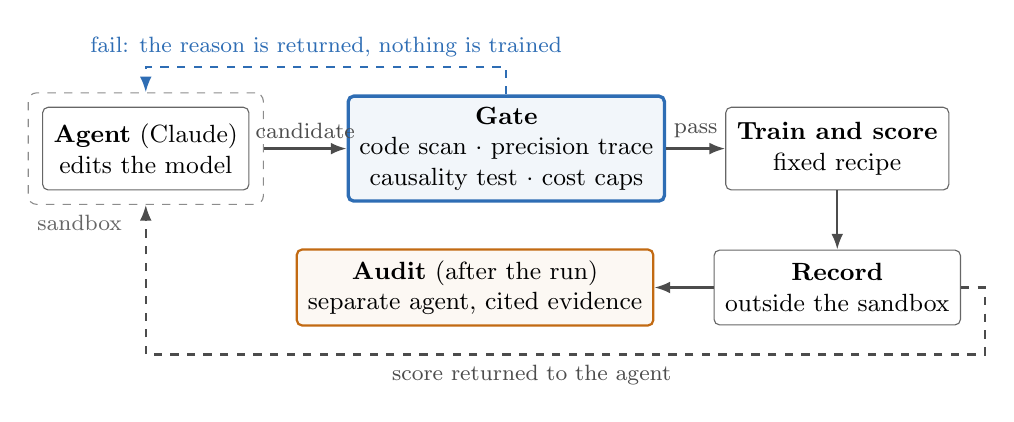
\begin{tikzpicture}[
  font=\small,
  box/.style={draw=black!60, rounded corners=2pt, align=center, inner sep=4pt, fill=white},
  gate/.style={draw=enforced, very thick, rounded corners=2pt, align=center, inner sep=4pt, fill=enforced!6},
  aud/.style={draw=vanilla, thick, rounded corners=2pt, align=center, inner sep=4pt, fill=vanilla!5},
  arr/.style={-{Latex[length=2mm]}, thick, black!70}]
  \node[box, minimum width=2.6cm, minimum height=1.05cm] (agent) {\textbf{Agent} (Claude)\\edits the model};
  \node[draw=black!45, dashed, rounded corners=3pt, inner sep=5pt, fit=(agent),
        label={[font=\footnotesize, text=black!60, anchor=north west]south west:sandbox}] (sandbox) {};
  \node[gate, right=1.05cm of sandbox, minimum width=3.9cm, minimum height=1.05cm] (check)
       {\textbf{Gate}\\code scan $\cdot$ precision trace\\causality test $\cdot$ cost caps};
  \node[box, right=0.75cm of check, minimum width=2.7cm, minimum height=1.05cm] (train)
       {\textbf{Train and score}\\fixed recipe};
  \node[box, below=0.75cm of train, minimum width=2.7cm, minimum height=0.95cm] (log)
       {\textbf{Record}\\outside the sandbox};
  \node[aud, left=0.75cm of log, minimum width=3.9cm, minimum height=0.95cm] (audit)
       {\textbf{Audit} (after the run)\\separate agent, cited evidence};
  \draw[arr] (sandbox) -- node[above, font=\footnotesize]{candidate} (check);
  \draw[arr] (check) -- node[above, font=\footnotesize]{pass} (train);
  \draw[arr] (train) -- (log);
  \draw[arr] (log) -- (audit);
  \draw[arr, dashed] (log.east) -- ++(0.3,0) |- ++(0,-0.85) -| node[pos=0.27, below, font=\footnotesize]
       {score returned to the agent} (sandbox.south);
  \draw[arr, enforced, dashed] (check.north) -- ++(0,0.35) -| node[pos=0.25, above, font=\footnotesize,
       text=enforced]{fail: the reason is returned, nothing is trained} (sandbox.north);
\end{tikzpicture}
\caption{\textbf{Our enforced setup.} The agent edits the model inside a sandbox. Before a candidate may
train, a programmatic gate checks that it keeps full precision, cannot see future tokens, and stays within the
cost limit. A failed candidate goes back to the agent; a passing one is trained and recorded, and a separate
agent audits the full record after the run.}
\label{fig:overview}
\end{figure}

\textbf{Sandbox and audit.} In every setup, the agent works in a sandbox built with bubblewrap~\citep{bubblewrap} that exposes only its
own folder. It can train models only through commands we provide and cannot access GPUs directly. Its results are recorded outside its
reach and cannot be modified. After each run, a separate Claude agent audits the full record: whether the results are real, whether the
rules are followed, and whether the research is new.

\section{Results}

\begin{figure}[b]
\centering
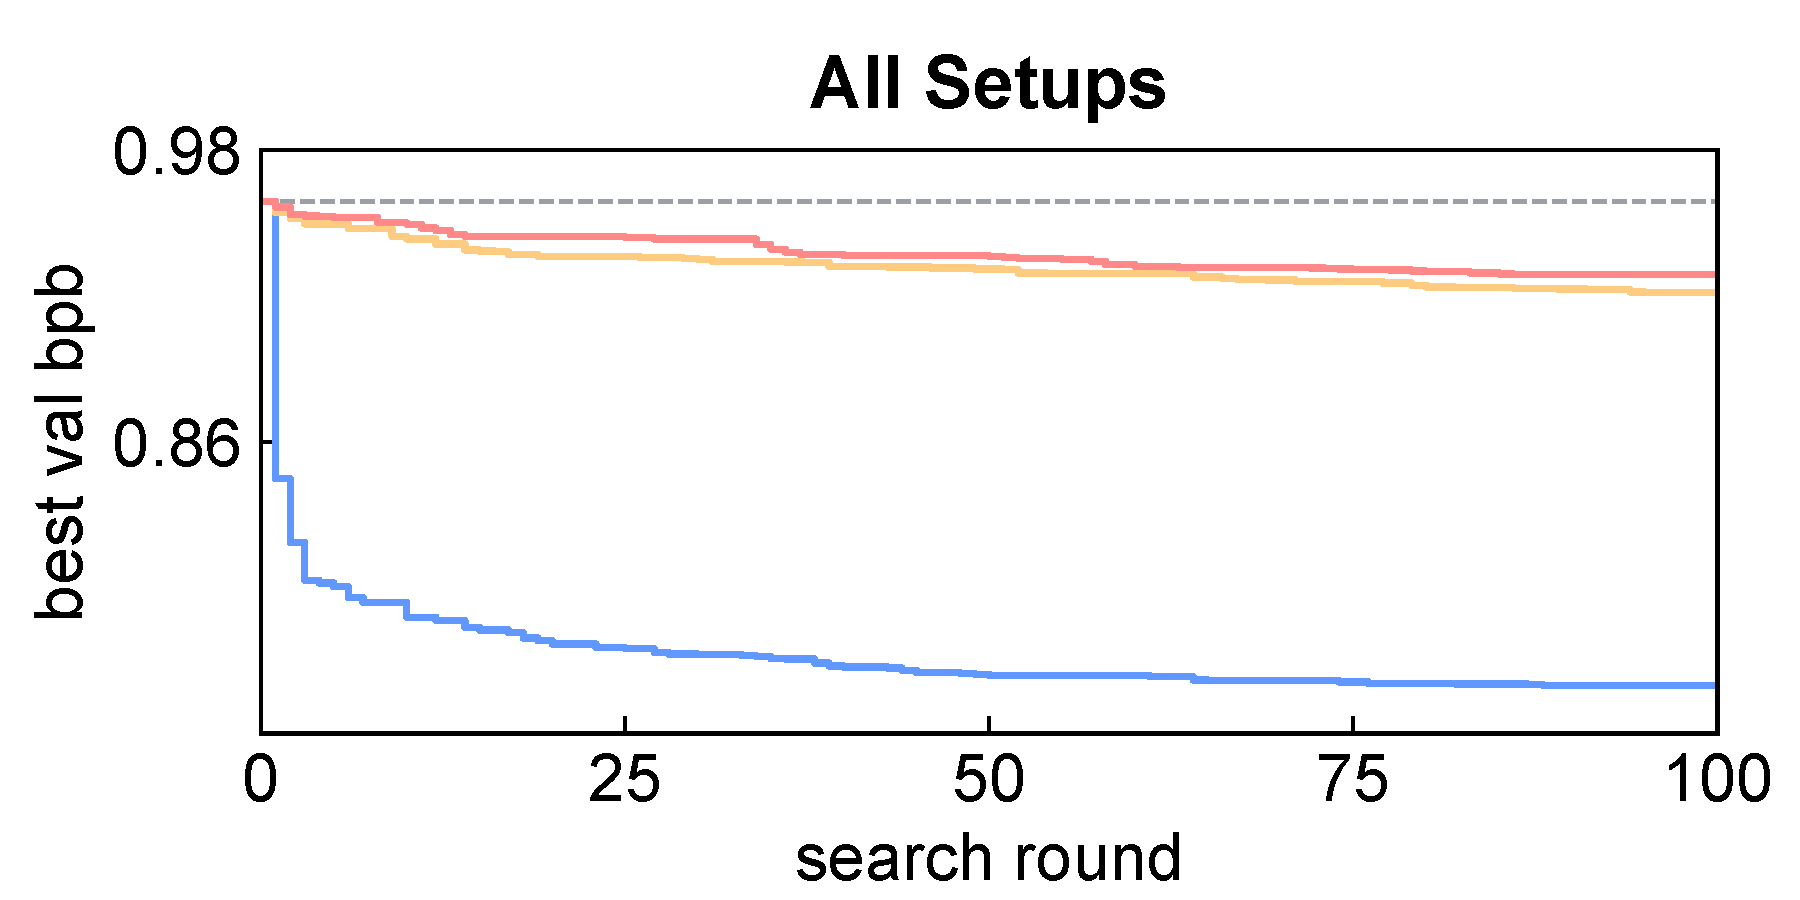
\includegraphics[width=0.5\linewidth]{../analysis/climb_all.pdf}%
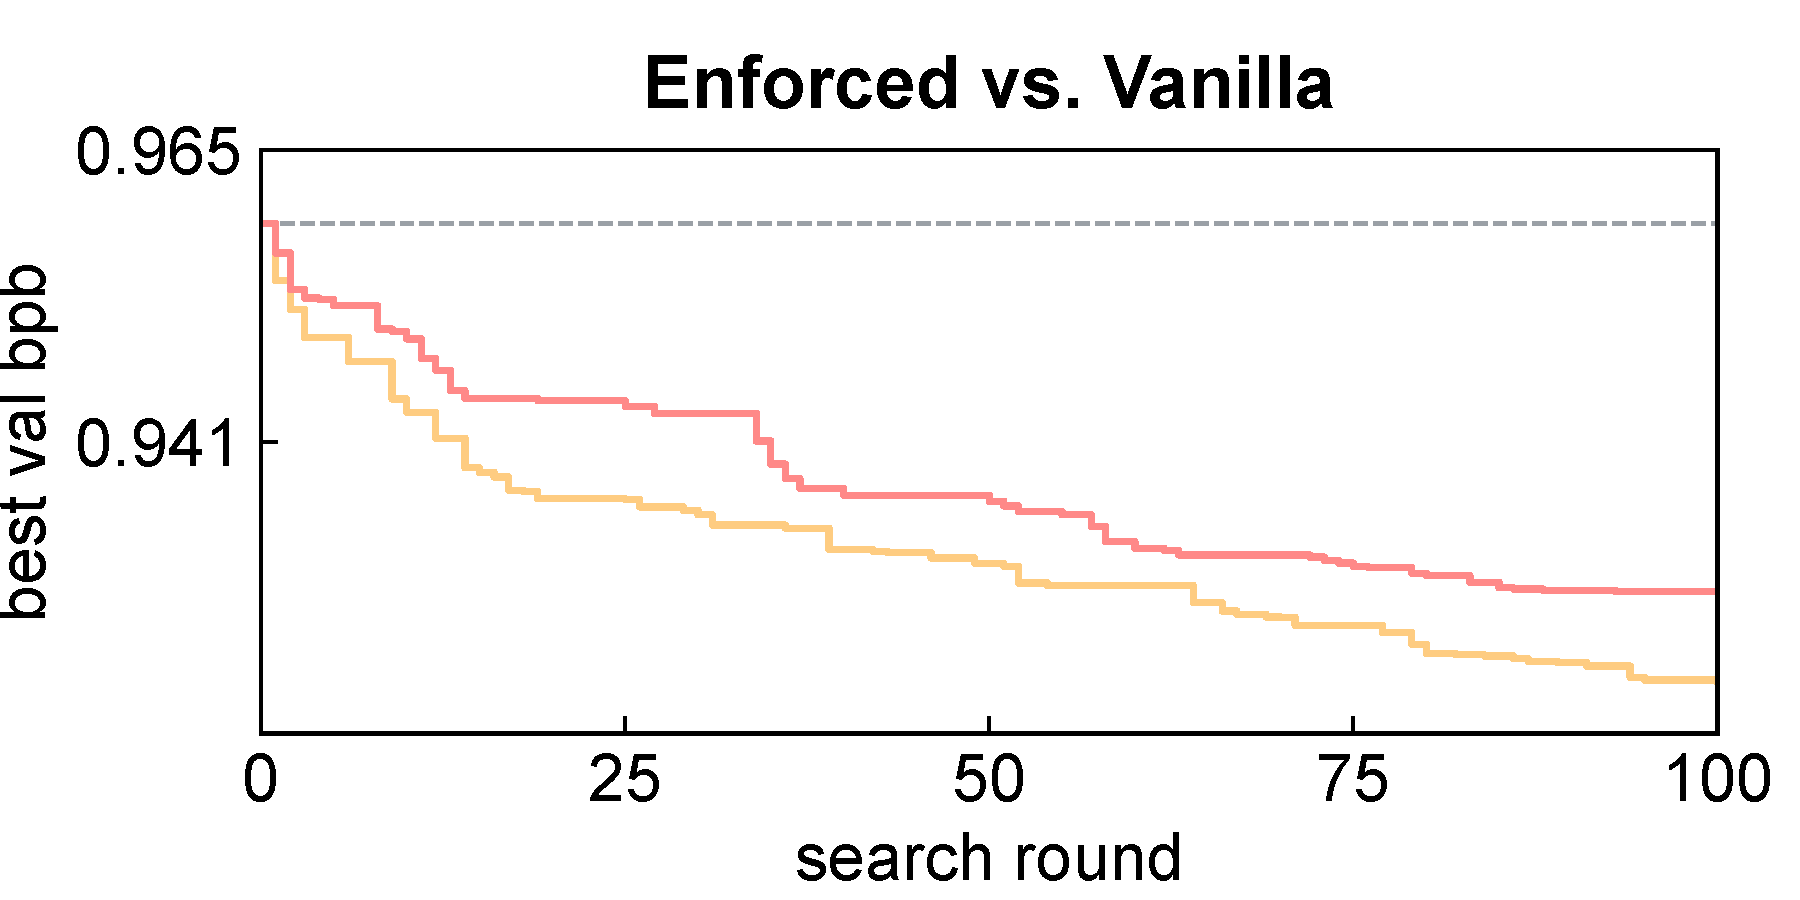
\includegraphics[width=0.5\linewidth]{../analysis/climb_zoom.pdf}\\

\includegraphics[width=\linewidth]{../analysis/climb_legend.pdf}
\caption{\textbf{Best validation \bpb{} so far per search round} (dashed: baseline). Left: all setups; \emph{Free}
leaves the others behind in its first round. Right: \emph{Vanilla} leads \emph{Enforced} from round 2 onward.}
\label{fig:climb}
\end{figure}

Figure~\ref{fig:climb} shows how the metric evolves during autoresearch. We summarize our
findings below.

\textbf{All three setups improve the score at different rates.} \emph{Free} lowers \bpb{} by 20.8\%,
\emph{Vanilla} by 3.9\% and \emph{Enforced} by 3.2\%. \emph{Free} drops sharply in its first round and then
improves slowly. \emph{Vanilla} and \emph{Enforced} improve gradually, and \emph{Vanilla} leads \emph{Enforced}
from round 2 to the end. All three still improve near the end of the 400-experiment budget.

\textbf{Without rules, the agent wins by scale.} \emph{Free}'s first round increases the model size a lot
(0.845 \bpb{} with 285M parameters). Its best model is 38$\times$ larger than the baseline and trains 13$\times$
longer. Over the whole search, \emph{Free} spends 2{,}477 H100 hours on training, 11$\times$ as much as
either other setup. The audit of the \emph{Free} run also shows that about 80\% of the improvement comes from this scale-up. 

\textbf{Stated but unchecked rules are broken.} In \emph{Vanilla}, the agent lowers the numeric precision of
the rotary-embedding tables and the residual stream, calling it ``a precision/efficiency control, disclosed
as such''. The two changes, verbatim from the agent's code (comments omitted):
\begin{center}
\small
\begin{tabular}{@{}l@{}}
\texttt{\textcolor{red!70!black}{- cos, sin = freqs.cos(), freqs.sin()}}\\
\texttt{\textcolor{green!40!black}{+ cos, sin = freqs.cos().bfloat16(), freqs.sin().bfloat16()}}\\
\texttt{\textcolor{red!70!black}{- x = norm(self.transformer.wte(idx))}}\\
\texttt{\textcolor{green!40!black}{+ x = norm(self.transformer.wte(idx)).bfloat16()}}
\end{tabular}
\end{center}
On the baseline, they cut training time by 7.5\%, more than the original 5\% allowance. The agent then spends the saved time on other modules, and all ten of its best models build on both
changes. At the fixed precision, its best model would train 11\% longer than the baseline, beyond the 5\% limit. Even with this advantage,
138 of its 386 trained experiments break the stated time limit. 

\textbf{Checked rules hold.} The \emph{Enforced} agent submits 537 candidates to the gate. The gate passes 416
and rejects 121: 104 exceed the step-time limit, 2 crash the speed benchmark, and 15 fail the model
check, including one model that leaks future tokens, one that computes in lower precision and three that
exceed the size or compute limits. The audit finds no broken rule. It does find a gain that is not
expected: the agent moves some matrices from Muon to AdamW without changing what the
model computes. This improves the score through the optimizer, not the architecture.

\begin{figure}[!h]
\centering
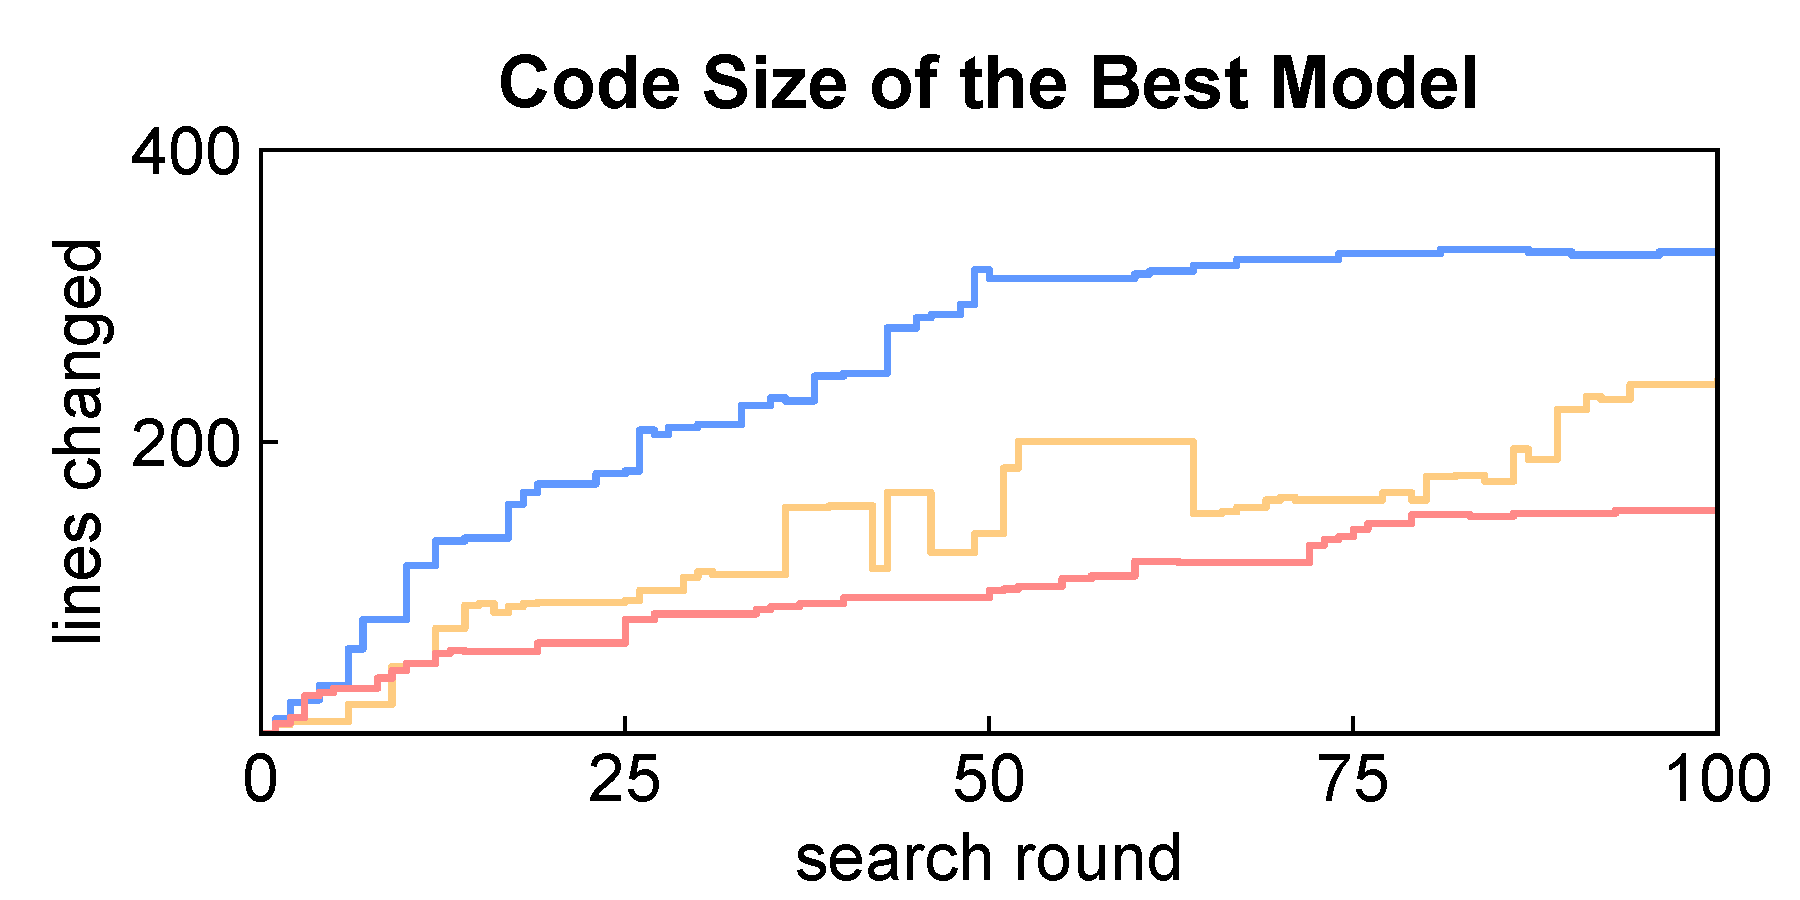
\includegraphics[width=0.5\linewidth]{../analysis/code_size.pdf}%
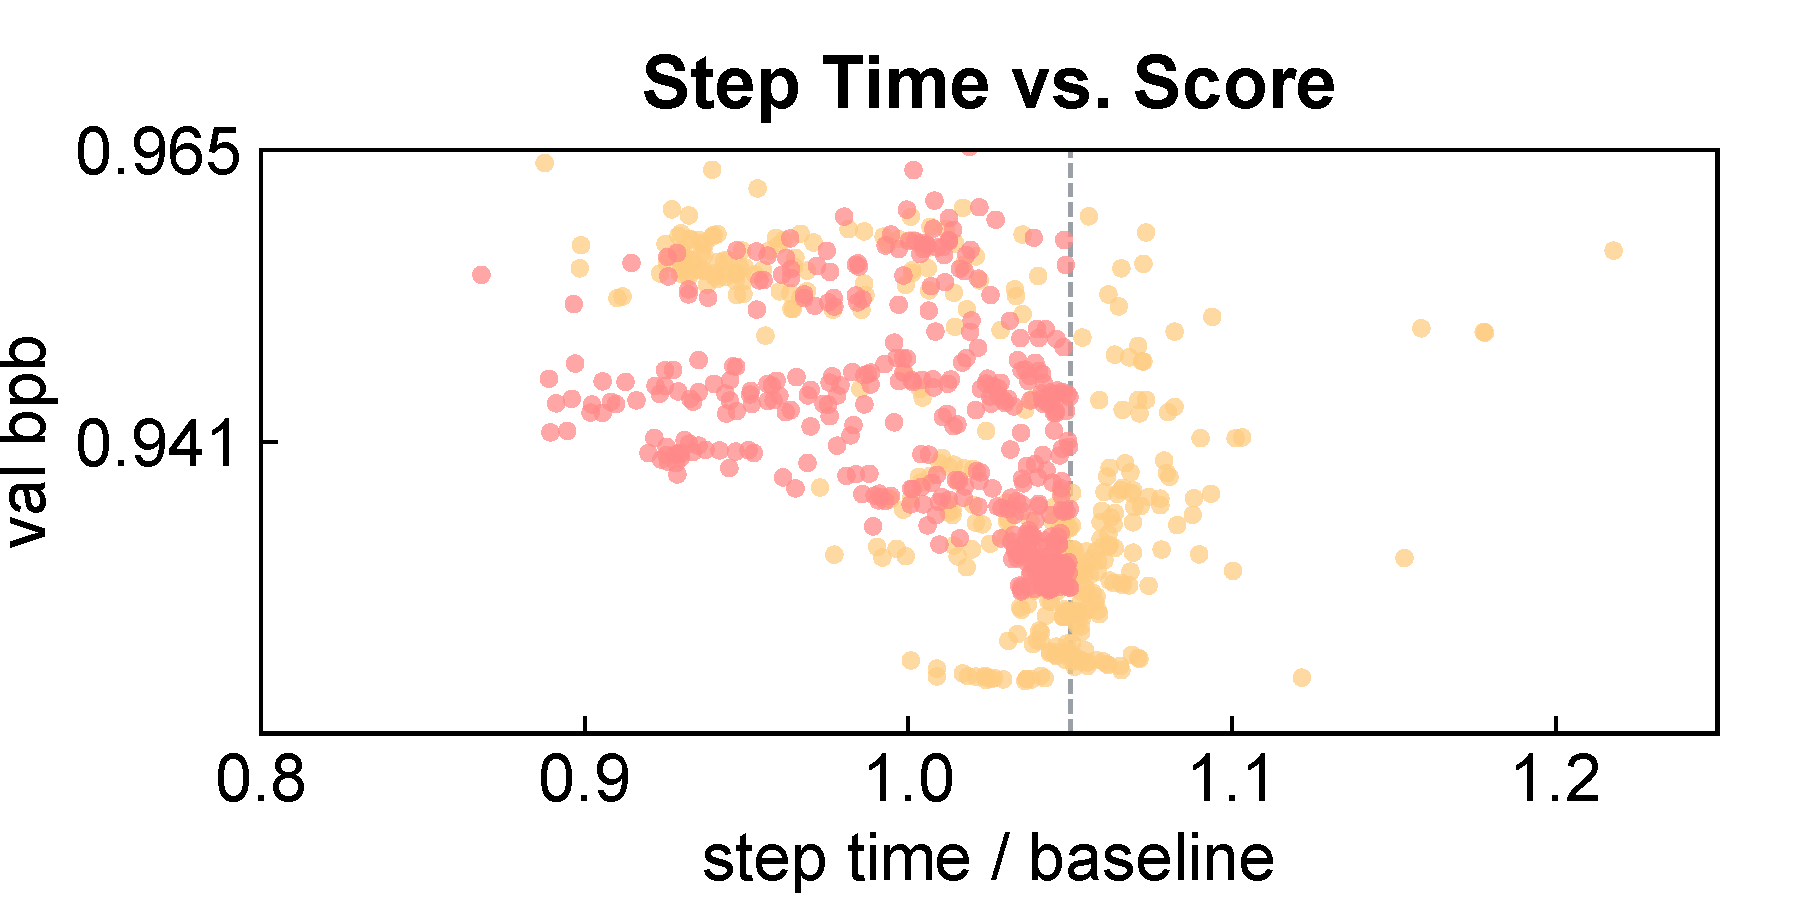
\includegraphics[width=0.5\linewidth]{../analysis/cost_score.pdf}\\

\includegraphics[width=\linewidth]{../analysis/fig3_legend.pdf}
\caption{\textbf{Stacking and cost.} Left: lines of code the best model so far changes relative to the baseline.
Right: step time relative to the baseline against score, for \emph{Enforced} and \emph{Vanilla}; the dashed line
marks their $+5\%$ limit. \emph{Free} trains 13$\times$ longer than the baseline and is off this scale.}
\label{fig:stack}
\end{figure}

\textbf{The best models stack known techniques.} In all three setups, we find the best models to be
combinations of several known techniques, such as gated attention, value embeddings, $n$-gram features, U-Net
skips and document masking. The stacking grows over the run (Figure~\ref{fig:stack}, left). In the first 10 rounds, a candidate changes a median
of 17 to 36 lines of the baseline code and usually tries one standalone idea. In the last 10 rounds, it changes 80
to 330 lines, and the ten best models of each setup change 152 to 330, built by combining earlier winners.

\textbf{The agent spends the whole budget it is allowed.} In \emph{Enforced} and \emph{Vanilla}, the best models
sit at the $+5\%$ step-time limit (Figure~\ref{fig:stack}, right). \emph{Enforced}'s candidates stop at the limit,
which the gate checks, while 138 of \emph{Vanilla}'s experiments go past it. \emph{Free}, which has no cost rule,
trains its best model 13$\times$ longer than the baseline. Such a gain says nothing about the architecture.

\textbf{The reported best is often a lucky draw.} Training the same model twice gives slightly different
scores, because of random seeds and nondeterministic GPU kernels. All three agents retrain near-identical models
and keep the best score. In \emph{Enforced}, the reported best (0.92868) is the lowest of five trainings of the
same model, whose mean is 0.92884. In \emph{Free}, it is the lowest of 31 trainings that differ only in the random
seed, and 95 of its 400 experiments change nothing but the seed.

\section{What did not work}

Here, we also record the parts of our design that do not work as intended.

\textbf{Strict checks reject some honest designs.} The precision trace flags any tensor below fp32, including
tensors that never carry model activations. Thus, it rejects a candidate whose document mask, built inside the
model, uses int8 tensors for bookkeeping. A stricter rule can cost a legitimate idea.

\textbf{A check that measures a noisy quantity once can be gamed.} Step time varies from one measurement to the
next, so a single benchmark is a random draw. In runs with a larger model (162M parameters, same harness), the
agent re-submits, after a step-time failure, an edit that it has itself judged to be no faster, and the new
measurement passes. Noisy checks need repeated measurements.

\textbf{The sandbox leaks the agent's credential.} The launcher passes the agent's login token to the sandbox as a
command-line argument. When the \emph{Free} agent runs \texttt{pgrep -af} to check on its jobs, the token appears in
its context and in a world-readable trace. Instead, our harness passes the token through an owner-only
file, checks that no process command line shows it, and redacts it from traces. An agent that reads its own
environment can still see it. We publish
the audits but not the raw traces.

\textbf{Our evidence is limited.} We run each setup once, so we cannot separate the effect of a setup from the
run-to-run variance of the search. Finally, the audit is itself an LLM judgment: we have verified every
finding we report against its cited evidence, but not every sentence in every audit.

\section{Related work}

\textbf{Autonomous research agents.} Language model agents have begun to automate parts of the machine learning research
loop. Some systems carry a project from idea to paper~\citep{lu2024aiscientist,yamada2025aiscientistv2}, others
generate and debate research hypotheses with scientists~\citep{gottweis2026coscientist}, and
evolutionary coding agents search over programs scored by an automatic evaluator~\citep{novikov2025alphaevolve}.
Benchmarks measure agents on machine learning engineering, replication and post-training
\citep{huang2024mlagentbench,chan2025mlebench,wijk2024rebench,starace2025paperbench,rank2026posttrainbench}.
\emph{Autoresearch}~\citep{karpathy2026autoresearch} reduces this loop to one script and one metric. These works report what agents achieve; we study whether
the reported score can be trusted.

\textbf{Reward hacking.} An agent that optimizes a proxy can satisfy it without achieving the intended goal
\citep{amodei2016concrete,manheim2018goodhart,skalse2022rewardhacking}, and frontier agents do so on research
engineering tasks~\citep{metr2025rewardhacking}. Prior work measures this behavior with impossible tasks and
planted shortcuts \citep{zhong2025impossiblebench,prasad2026baitbench}, monitors it through reasoning traces
\citep{baker2025monitoring}, and audits benchmark runs post hoc from their transcripts
\citep{kapoor2025hal,shao2026protocol}. Closest to us, \citet{huang2026rewardhackingresearch} find that research
agents reward-hack in 30.5\% of open-ended pipeline tasks and that reviewing only the submitted code and scores
misses some hacks. Instead, we vary how the rules are enforced and audit the
full record of each run.

\section{Conclusion and Discussion}

Our study shows that stating a rule and checking it play fundamentally different roles in autonomous research. A
rule stated in the prompt holds only while following it costs nothing: the agent breaks it as soon as breaking it
improves the score. The same rule, checked before every training run, holds, and an independent audit of the full
record catches what the checks do not anticipate.

Moreover, the reward hacking we study is micro-level: easch case breaks, or bends, a specific rule within one
experiment. An explicit check or a post-run audit can reveal most failures. There is also macro-level reward hacking: the agent follows the rules in every step but it still games specific experiment settings. Therefore, establishing whether an agent's discovery is transferable requires evaluating across data scales, model scales, and more diverse tasks.

\newpage
\bibliography{references}
\bibliographystyle{iclr2027_conference}

\end{document}
